Miguel tiene bloques de plástico de igual tamaño y arma una torre con todos ellos. Observa la figura \ref{fig:22bc4d835622314209af99a305ea2515952e3902}:\\

\begin{minipage}{0.35\textwidth}
    \begin{figure}[H]
        \centering
        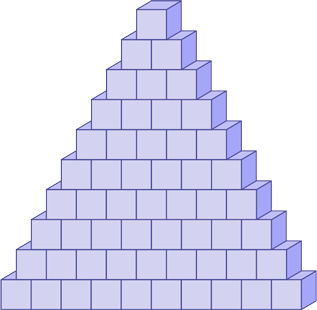
\includegraphics[width=0.7\linewidth]{../images/22bc4d835622314209af99a305ea2515952e3902}
        \caption{Torre con bloques.}
        \label{fig:22bc4d835622314209af99a305ea2515952e3902}
    \end{figure}
\end{minipage}\hfill
\begin{minipage}{0.6\textwidth}
    Si Miguel armara una torre de 32 filas,
    \textbf{¿cuántos bloques necesitará en total?}\\
    \begin{solutionbox}{5cm}
        Ya que la regla de recurrencia es:
        \[a_n=(n-1)+1\]
        entonces,
        \[a_{32}=(32-1)+1=32\]
        y,
        \[s_{32}=\dfrac{32(a_0+a_{32})}{2}=\dfrac{32(1+32)}{2}=528\]
    \end{solutionbox}
\end{minipage}